\documentclass[13pt,a4paper]{article}

% --- CÁC THƯ VIỆN BẮT BUỘC ---
\usepackage[utf8]{inputenc} % Hỗ trợ gõ Unicode
\usepackage[T5]{fontenc}    % Hỗ trợ hiển thị tiếng Việt
\usepackage{amsmath}        % Thư viện toán học cốt lõi (cho ngoặc, ma trận)
\usepackage{amssymb}        % Thư viện ký hiệu toán học
\usepackage{amsfonts}       % Font chữ toán học
\usepackage[margin=2.5cm]{geometry} % Căn lề chuẩn báo cáo
\usepackage{graphicx} % Thư viện dùng để chèn ảnh
\usepackage{float}
\usepackage{listings}
\usepackage{xcolor}
\definecolor{codegreen}{rgb}{0,0.6,0}
\definecolor{codegray}{rgb}{0.5,0.5,0.5}
\definecolor{codepurple}{rgb}{0.58,0,0.82}
\definecolor{backcolour}{rgb}{0.95,0.95,0.92}

\lstdefinestyle{mystyle}{
    backgroundcolor=\color{backcolour},   
    commentstyle=\color{codegreen},
    keywordstyle=\color{magenta},
    numberstyle=\tiny\color{codegray},
    stringstyle=\color{codepurple},
    basicstyle=\ttfamily\footnotesize,
    breakatwhitespace=false,         
    breaklines=true,                 
    captionpos=b,                    
    keepspaces=true,                 
    numbers=left,                    
    numbersep=5pt,                  
    showspaces=false,                
    showstringspaces=false,
    showtabs=false,                  
    tabsize=4
}
\lstset{style=mystyle}
\begin{document}
% ================= BÌA =================
\begin{titlepage}
    \begin{center}
        {\Large \textbf{ĐẠI HỌC PHENIKAA}} \\[0.2cm]
        {\Large \textbf{TRƯỜNG CÔNG NGHỆ THÔNG TIN PHENIKAA}} \\[2cm]
        
        % Bỏ comment dòng dưới nếu bạn có file ảnh logo và muốn chèn vào
        % \includegraphics[width=6cm]{logo_phenikaa.png} \\[2cm]
        
        {\large \textbf{TÊN HỌC PHẦN: NHẬP MÔN TRÍ TUỆ NHÂN TẠO}} \\[1.5cm]
        
        {\Large \textbf{TÊN ĐỀ TÀI:}} \\[0.5cm]
        {\Large \textbf{CÀI ĐẶT PERCEPTRON VÀ MẠNG NƠ-RON NHIỀU LỚP (MLP) TỪ ĐẦU BẰNG NUMPY}} \\[2.5cm]
    \end{center}

    \begin{flushleft}
        \large
        \textbf{Giảng viên hướng dẫn:} ThS. Phan Thị Hoài \\[0.5cm]
        \textbf{Sinh viên thực hiện \hspace{0.1cm}:} Ngô Quang Thiện - 24102651 \\
        \hspace{4.8cm} Nguyễn Hưng Vũ - 24102769 \\[0.5cm]
        \textbf{Khoá \hspace{2.9cm}:} K18 - ICT3 \\
        \textbf{Lớp tín chỉ \hspace{1.7cm}:} CSE703041-2-3-25(N02) \\
        \textbf{Chương trình đào tạo:} Khoa Học Dữ Liệu và Trí Tuệ Nhân Tạo \\
    \end{flushleft}
    
    \vfill
    \begin{center}
        \textbf{Hà Nội, tháng 7 năm 2026}
    \end{center}
\end{titlepage}
% --- KẾT THÚC TRANG BÌA ---
\newpage % Ngắt trang bìa sang trang mới

% --- MỤC LỤC ---
\renewcommand{\contentsname}{\begin{center} MỤC LỤC \end{center}}
\tableofcontents
\newpage

% --- DANH MỤC HÌNH ẢNH ---
\renewcommand{\listfigurename}{\begin{center} DANH MỤC HÌNH ẢNH \end{center}}
\listoffigures
\newpage
% ================= CHƯƠNG 1 =================
\section*{CHƯƠNG 1: MỞ ĐẦU}
\addcontentsline{toc}{section}{CHƯƠNG 1: MỞ ĐẦU}

\subsection*{1.1. Đặt vấn đề}
\addcontentsline{toc}{subsection}{1.1. Đặt vấn đề}
Trong những năm gần đây, Trí tuệ nhân tạo (AI) và Học sâu (Deep Learning) đã đạt được những bước tiến vượt bậc, ứng dụng sâu rộng vào nhiều lĩnh vực từ nhận dạng hình ảnh, xử lý ngôn ngữ tự nhiên đến hệ thống tự động hóa. Hiện nay, các thư viện và framework mạnh mẽ như TensorFlow hay PyTorch cho phép các lập trình viên xây dựng một mô hình AI phức tạp chỉ với vài dòng mã lệnh.

Tuy nhiên, sự tiện lợi này vô tình biến các mạng nơ-ron trở thành những "hộp đen" (black boxes). Việc lạm dụng các công cụ có sẵn mà thiếu đi sự thấu hiểu về bản chất toán học, luồng xử lý bộ nhớ và cách thức các ma trận tương tác ở tầng thấp sẽ tạo ra rào cản lớn khi cần tối ưu hóa thuật toán hoặc giải quyết các bài toán đặc thù. Do đó, việc quay trở lại với những nguyên lý nền tảng, tự tay xây dựng các cấu trúc dữ liệu và logic toán học từ con số không là một bước đi cần thiết để làm chủ công nghệ này.

\subsection*{1.2. Mục tiêu đề tài}
\addcontentsline{toc}{subsection}{1.2. Mục tiêu đề bài}
Đồ án này được thực hiện với mục tiêu phá vỡ "hộp đen" của mạng nơ-ron nhân tạo thông qua việc tự thiết kế và lập trình một hệ thống Mạng nơ-ron nhiều lớp (Multi-Layer Perceptron - MLP) hoàn toàn bằng toán học ma trận. Thay vì sử dụng các hàm có sẵn, hệ thống sẽ được cấu trúc theo mô hình Lập trình Hướng đối tượng (OOP), đảm bảo tính module hóa cao và tối ưu tốc độ tính toán phần cứng thông qua kỹ thuật vector hóa.

Các mục tiêu cụ thể bao gồm:
\begin{itemize}
    \item Hiểu và cài đặt thành công thuật toán Lan truyền thuận (Forward Propagation) và Lan truyền ngược (Backpropagation) dựa trên quy tắc chuỗi (Chain Rule).
    \item Phân tích toán học và trực quan hóa giới hạn của mạng nơ-ron đơn lớp thông qua bài toán XOR.
    \item Đánh giá hiệu suất của các thuật toán tối ưu (SGD, Momentum) và kỹ thuật chống học vẹt (L2 Regularization) trên tập dữ liệu thực tế.
\end{itemize}

\subsection*{1.3. Phạm vi nghiên cứu}
\addcontentsline{toc}{subsection}{1.3. Phạm vi nghiên cứu}
Đồ án tập trung nghiên cứu kiến trúc mạng kết nối đầy đủ (Fully Connected Neural Networks). Mã nguồn cốt lõi không sử dụng bất kỳ framework học sâu nào, chỉ giới hạn sử dụng thư viện NumPy để tính toán ma trận. Mô hình sẽ được đánh giá trên hai tập dữ liệu tĩnh có kích thước nhỏ và vừa: bài toán phân loại logic nhị phân (XOR Dataset) và bài toán phân loại đa lớp (Iris Dataset).

\section*{CHƯƠNG 2: CƠ SỞ LÝ THUYẾT}
\addcontentsline{toc}{section}{CHƯƠNG 2: CỞ SỞ LÝ THUYẾT}
\subsection*{2.1. Mạng Perceptron một lớp và Giới hạn phân tách tuyến tính}
\addcontentsline{toc}{subsection}{2.1. Mạng Perceptron một lớp và Giới hạn phân tách tuyến tính}
Perceptron là mô hình tính toán mô phỏng lại một nơ-ron sinh học, được Frank Rosenblatt giới thiệu vào năm 1957. Cấu trúc của Perceptron nhận một vector dữ liệu đầu vào $\mathbf{x} = [x_1, x_2, \dots, x_n]$, sau đó thực hiện phép tính tổng trọng số và cộng thêm một độ lệch $b$ (bias).

Phương trình tuyến tính tại nơ-ron được biểu diễn như sau:
\[
z = \sum_{i=1}^{n} w_i x_i + b = \mathbf{w}^T \mathbf{x} + b
\]

Kết quả $z$ sau đó được đưa qua một hàm kích hoạt $f(z)$ (thường là hàm bước nhảy - Step function) để đưa ra dự đoán nhị phân $\hat{y} \in \{0, 1\}$. Quá trình huấn luyện Perceptron là quá trình điều chỉnh vector $\mathbf{w}$ và $b$ để tìm ra một "siêu mặt phẳng" (hyperplane) chia tách hai lớp dữ liệu.

Tuy nhiên, Perceptron gặp phải một giới hạn toán học nghiêm trọng: nó chỉ có thể giải quyết các bài toán phân tách tuyến tính (linearly separable). Điển hình là hàm logic XOR, nơi dữ liệu mang giá trị $1$ khi hai đầu vào trái ngược nhau và mang giá trị $0$ khi chúng giống nhau. Không tồn tại bất kỳ một đường thẳng nào trên không gian 2D có thể chia tách hoàn hảo 4 điểm dữ liệu của hàm XOR, dẫn đến sự thất bại của mô hình đơn lớp này.

\subsection*{2.2. Mạng nơ-ron nhiều lớp (MLP)}
\addcontentsline{toc}{subsection}{2.2. Mạng nơ-ron nhiều lớp (MLP)}
Để giải quyết bài toán phi tuyến, Mạng nơ-ron nhiều lớp (MLP) được sử dụng. MLP chèn thêm một hoặc nhiều "lớp ẩn" (hidden layers) nằm giữa đầu vào và đầu ra, kết hợp với các hàm kích hoạt phi tuyến để uốn nắn không gian dữ liệu.

\textbf{Lan truyền thuận (Forward Propagation):} \\
Quá trình tính toán kết quả từ lớp đầu vào đến đầu ra được gọi là lan truyền thuận. Tại lớp thứ $l$, ma trận giá trị $Z^{(l)}$ và đầu ra $A^{(l)}$ được tính toán thông qua các phép nhân ma trận:
\[
Z^{(l)} = W^{(l)} A^{(l-1)} + b^{(l)}
\]
\[
A^{(l)} = f^{(l)}(Z^{(l)})
\]
(Trong đó, $A^{(0)} = X$ là ma trận dữ liệu đầu vào, $W^{(l)}$ là ma trận trọng số của lớp $l$).

\textbf{Hàm mất mát (Loss Function):} \\
Để đánh giá mô hình dự đoán sai lệch bao nhiêu so với thực tế, ta sử dụng hàm mất mát. Với bài toán phân loại nhị phân, hàm Binary Cross-Entropy thường được áp dụng:
\[
L = -\frac{1}{m} \sum_{i=1}^{m} \left( y_i \log(\hat{y}_i) + (1 - y_i) \log(1 - \hat{y}_i) \right)
\]

\textbf{Lan truyền ngược (Backpropagation):} \\
Lan truyền ngược là thuật toán tính toán độ dốc (gradient) của hàm mất mát theo từng phần tử trọng số trong mạng, làm cơ sở để cập nhật chúng. Thuật toán này sử dụng Quy tắc chuỗi (Chain Rule) trong giải tích.

Để tính đạo hàm của hàm mất mát $L$ theo trọng số $W^{(l)}$ tại lớp $l$, ta có công thức:
\[
\frac{\partial L}{\partial W^{(l)}} = \frac{\partial L}{\partial Z^{(l)}} \cdot \frac{\partial Z^{(l)}}{\partial W^{(l)}} = dZ^{(l)} \cdot (A^{(l-1)})^T
\]

Vector sai số $dZ^{(l)}$ được truyền lùi từ lớp $l+1$ phía sau nó:
\[
dZ^{(l)} = (W^{(l+1)})^T dZ^{(l+1)} * f'(Z^{(l)})
\]
(Ký hiệu $*$ là phép nhân từng phần tử - element-wise multiplication).

\subsection*{2.3. Các thuật toán Tối ưu hóa (Optimizers)}
\addcontentsline{toc}{subsection}{2.3. Các thuật toán Tối ưu hóa (Optimizers)}
Sau khi có được ma trận gradient $\nabla W = \frac{\partial L}{\partial W}$, mô hình cần một thuật toán để cập nhật lại các trọng số này.

\textbf{Stochastic Gradient Descent (SGD):} Cập nhật trọng số theo hướng ngược lại với chiều của gradient.
\[
W_{t+1} = W_t - \eta \nabla W_t
\]
(Với $\eta$ là tốc độ học - learning rate).

\textbf{SGD with Momentum:} Trong thực tế, hàm mất mát thường có nhiều khe hẹp và điểm cực tiểu cục bộ, khiến SGD thuần bị dao động mạnh (răng cưa). Thuật toán Momentum mô phỏng lực quán tính trong vật lý bằng cách cộng dồn một phần hướng đi của bước trước đó vào bước hiện tại, giúp hội tụ nhanh và mượt mà hơn.
\[
v_t = \gamma v_{t-1} + \eta \nabla W_t
\]
\[
W_{t+1} = W_t - v_t
\]
(Với $\gamma$ là hệ số momentum, thường chọn bằng $0.9$).

\subsection*{2.4. Khắc phục Overfitting với L2 Regularization}
\addcontentsline{toc}{subsection}{2.4. Khắc phục Overfitting với L2 Regularization}
Khi mạng nơ-ron có quá nhiều tham số nhưng số lượng dữ liệu huấn luyện lại khiêm tốn (ví dụ tập Iris), mô hình sẽ có xu hướng "học vẹt" (Overfitting). Mô hình khớp hoàn hảo với dữ liệu huấn luyện nhưng dự đoán rất tệ trên dữ liệu mới.

Kỹ thuật L2 Regularization (hay Weight Decay) khắc phục điều này bằng cách thêm một hình phạt tỷ lệ thuận với bình phương độ lớn của các trọng số vào hàm mất mát tổng:
\[
L_{total} = L + \frac{\lambda}{2m} \sum_{l=1}^{L} \|W^{(l)}\|_2^2
\]
Khi tính toán lan truyền ngược, thành phần cập nhật trọng số sẽ tự động bị giảm trừ đi một lượng nhỏ $\frac{\lambda}{m} W^{(l)}$, ép các trọng số phân bố đều và có giá trị nhỏ, từ đó triệt tiêu sự phụ thuộc quá mức vào một vài nơ-ron nhất định.

\section*{CHƯƠNG 3: CÀI ĐẶT HỆ THỐNG}
\addcontentsline{toc}{section}{CHƯƠNG 3: CÀI ĐẶT HỆ THỐNG}
\subsection*{3.1. Thiết kế kiến trúc Hướng đối tượng (OOP)}
\addcontentsline{toc}{subsection}{3.1. Thiết kế kiến trúc Hướng đối tượng (OOP)}
Để tránh việc mã nguồn trở thành một mớ hỗn độn (spaghetti code) khi số lượng lớp ẩn tăng lên, hệ thống được thiết kế theo mô hình Lập trình Hướng đối tượng (OOP). Mỗi thành phần toán học của mạng nơ-ron được đóng gói thành một lớp (Class) riêng biệt, tuân thủ nguyên tắc thiết kế module:

\begin{itemize}
    \item \textbf{Module Activation (Hàm kích hoạt):} Chứa các class như Sigmoid, ReLU, Softmax. Mỗi class bắt buộc phải có hai phương thức: \texttt{forward(Z)} để tính toán lan truyền thuận và \texttt{backward(Z)} để trả về đạo hàm tương ứng.
    \item \textbf{Class DenseLayer (Lớp kết nối đầy đủ):} Quản lý ma trận trọng số $W$ và vector độ lệch $b$. Lớp này đảm nhiệm việc thực hiện phép nhân ma trận ở pha thuận và áp dụng quy tắc chuỗi, kết hợp thuật toán tối ưu (SGD/Momentum) cùng L2 Regularization ở pha ngược.
    \item \textbf{Class MLP (Mô hình mạng nơ-ron):} Đóng vai trò là bộ điều khiển trung tâm (Controller). Class này lưu trữ danh sách các DenseLayer theo thứ tự, chứa hàm \texttt{fit()} để lặp qua các Epochs, duyệt tuần tự qua các lớp (forward) và duyệt ngược lại (backward) để huấn luyện.
\end{itemize}

\subsection*{3.2. Tiền xử lý dữ liệu (Data Preprocessing)}
\addcontentsline{toc}{subsection}{3.2. Tiền xử lý dữ liệu (Data Preprocessing)}
Mô hình được huấn luyện và kiểm thử trên hai tập dữ liệu với các kỹ thuật tiền xử lý tương ứng:

\begin{itemize}
    \item \textbf{Tập dữ liệu XOR:} Được khởi tạo tĩnh thông qua thư viện NumPy với ma trận đầu vào $X$ kích thước $(4, 2)$ và vector nhãn $y$ kích thước $(4, 1)$.
    \item \textbf{Tập dữ liệu Iris:} Gồm 150 mẫu hoa chia làm 3 lớp. Dữ liệu được xử lý qua 3 bước:
    \begin{itemize}
        \item \textit{Mã hóa nhãn (One-Hot Encoding):} Chuyển đổi nhãn phân lớp $[0, 1, 2]$ thành các vector xác suất, ví dụ lớp 0 thành $[1, 0, 0]$ để phù hợp với đầu ra của hàm Softmax.
        \item \textit{Chuẩn hóa (Standardization):} Sử dụng công thức $x' = \frac{x - \mu}{\sigma}$ để đưa các đặc trưng về phân phối chuẩn (trung bình bằng 0, phương sai bằng 1), giúp tránh hiện tượng bão hòa gradient (vanishing gradient).
        \item \textit{Chia tập dữ liệu:} Phân tách ngẫu nhiên thành $80\%$ dữ liệu huấn luyện (Train set) và $20\%$ dữ liệu kiểm thử (Test set).
    \end{itemize}
\end{itemize}

\subsection*{3.3. Tối ưu hóa tính toán bằng Vector hóa (Vectorization)}
\addcontentsline{toc}{subsection}{3.3. Tối ưu hóa tính toán bằng Vector hóa (Vectorization)}
Một trong những thách thức lớn nhất khi không sử dụng framework là tốc độ thực thi. Nếu sử dụng các vòng lặp \texttt{for} lồng nhau để duyệt qua từng nơ-ron và tính tổng trọng số, thời gian huấn luyện sẽ tăng theo cấp số nhân. Đồ án đã áp dụng triệt để kỹ thuật Vector hóa thông qua hàm \texttt{np.dot()} của NumPy. Kỹ thuật này ánh xạ các vòng lặp toán học xuống cấp độ mã máy (C/C++ backend) và tính toán ma trận song song, giảm thiểu thời gian huấn luyện một Epoch từ vài giây xuống chỉ còn vài mili-giây.
\subsection*{3.4. Trích xuất mã nguồn các hàm toán học cốt lõi}
\addcontentsline{toc}{subsection}{3.4. Trích xuất mã nguồn các hàm toán học cốt lõi}
Để làm rõ quá trình chuyển đổi từ công thức toán học lý thuyết sang mã lệnh thực thi, dưới đây là chi tiết cài đặt của hai thành phần quan trọng nhất trong mạng lưới: Hàm mất mát (Loss Function) và Thuật toán Lan truyền ngược (Backpropagation).

\textbf{1. Cài đặt Hàm mất mát Cross-Entropy} \\
Trong bài toán phân loại, hàm Cross-Entropy được ưu tiên sử dụng. Quá trình lập trình phải xử lý khéo léo lỗi toán học khi logarit nhận giá trị $0$ (thông qua hằng số epsilon).

\begin{lstlisting}[language=Python, caption=Cài đặt hàm Binary Cross-Entropy]
class BinaryCrossEntropyLoss:
    def forward(self, y_pred, y_true):
        # Them epsilon de tranh loi log(0) ra vo cuc (NaN)
        epsilon = 1e-15
        y_pred = np.clip(y_pred, epsilon, 1 - epsilon)
        
        # Cong thuc tinh Loss trung binh tren toan bo mini-batch
        loss = -np.mean(y_true * np.log(y_pred) + (1 - y_true) * np.log(1 - y_pred))
        return loss

    def backward(self, y_pred, y_true):
        epsilon = 1e-15
        y_pred = np.clip(y_pred, epsilon, 1 - epsilon)
        
        # Dao ham cua Cross-Entropy de truyen ve mang
        d_inputs = - (y_true / y_pred) + (1 - y_true) / (1 - y_pred)
        return d_inputs
\end{lstlisting}

\textbf{2. Cài đặt Thuật toán Lan truyền ngược tại DenseLayer} \\
Đây là "trái tim" của mô hình học máy. Phương thức \texttt{backward} tiếp nhận vector sai số \texttt{dZ} từ lớp phía sau, áp dụng Quy tắc chuỗi (Chain Rule) để tính đạo hàm trọng số, đồng thời tích hợp thuật toán tối ưu Momentum và thành phần phạt L2 Regularization. Việc tính toán 100\% sử dụng phép nhân ma trận (\texttt{np.dot}) để tận dụng tính năng Vector hóa.

\begin{lstlisting}[language=Python, caption=Cài đặt Lan truyền ngược (Backpropagation) và cập nhật trọng số]
def backward(self, dZ, learning_rate, optimizer='sgd', momentum=0.9):
    m = self.inputs.shape[0] # Lay so luong mau du lieu (batch size)

    # 1. Tinh Gradient cua W va b (Co cong them dao ham cua L2 Regularization)
    dW = np.dot(self.inputs.T, dZ) / m + (self.l2_lambda / m) * self.W
    db = np.sum(dZ, axis=0, keepdims=True) / m

    # 2. Tinh dao ham truyen nguoc cho lop phia truoc (Chain Rule)
    d_inputs = np.dot(dZ, self.W.T)

    # 3. Cap nhat trong so (Weights) theo thuat toan toi uu
    if optimizer == 'momentum':
        # Tinh toan quan tinh (Velocity)
        self.v_W = momentum * self.v_W + learning_rate * dW
        self.v_b = momentum * self.v_b + learning_rate * db
        
        # Tru di gradient
        self.W -= self.v_W
        self.b -= self.v_b
    else:
        # Cap nhat theo SGD co ban
        self.W -= learning_rate * dW
        self.b -= learning_rate * db

    return d_inputs
\end{lstlisting}
\section*{CHƯƠNG 4: ĐÁNH GIÁ KẾT QUẢ THỰC NGHIỆM}
\addcontentsline{toc}{section}{CHƯƠNG 4: ĐÁNH GIÁ KẾT QUẢ THỰC NGHIỆM}
\subsection*{4.1. Thực nghiệm 1: Giới hạn phân tách tuyến tính của Perceptron}
\addcontentsline{toc}{subsection}{4.1. Thực nghiệm 1: Giới hạn phân tách tuyến tính của Perceptron}
\textbf{Mục tiêu:} Chứng minh toán học thông qua thực nghiệm rằng Perceptron đơn lớp không thể giải quyết bài toán XOR.

\textbf{Kết quả phân tích:} Đồ thị phân tán (Scatter plot) cho thấy 4 điểm dữ liệu XOR nằm ở 4 góc chéo nhau. Đường ranh giới quyết định (Decision Boundary) do Perceptron học được là một đường thẳng. Dù trải qua hàng ngàn Epochs, đường thẳng này không thể nào chia tách hoàn toàn các điểm màu đỏ (nhãn 0) và màu xanh (nhãn 1), dẫn đến độ chính xác tối đa chỉ đạt 50\%.

\begin{figure}[H]
    \centering
    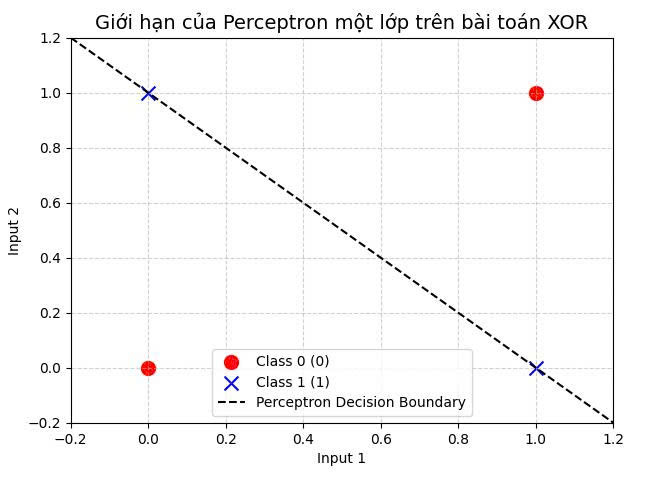
\includegraphics[width=0.75\textwidth]{17.jpg} 
    \caption{Giới hạn của Perceptron một lớp trên bài toán XOR.}
    \label{fig:xor_perceptron}
\end{figure}
\textbf{Phân tích chi tiết tọa độ và tỷ lệ lỗi:} 
Trên đồ thị không gian 2D, trục hoành (Input 1) và trục tung (Input 2) biểu diễn 4 trạng thái đầu vào của cổng logic XOR. Các điểm dữ liệu mang nhãn 0 (màu đỏ) nằm ở tọa độ $(0,0)$ và $(1,1)$, trong khi các điểm mang nhãn 1 (màu xanh) nằm ở tọa độ $(0,1)$ và $(1,0)$. 

Đường nét đứt màu đen biểu diễn ranh giới quyết định tuyến tính (phương trình $w_1x_1 + w_2x_2 + b = 0$) tốt nhất mà Perceptron có thể học được. Như đồ thị cho thấy, đường thẳng này chỉ có thể cô lập được tối đa một cụm điểm cùng màu ở một phía (ví dụ: điểm màu xanh ở tọa độ $(1,0)$), trong khi 3 điểm còn lại nằm lẫn lộn ở nửa mặt phẳng đối diện. Điều này giải thích tại sao độ chính xác cao nhất mà thuật toán đạt được bị kẹt ở mức $50\%$ (dự đoán đúng 2/4 mẫu). Mức sai số $50\%$ này là minh chứng toán học tuyệt đối cho giới hạn của mạng nơ-ron không có lớp ẩn.
\subsection*{4.2. Thực nghiệm 2: Huấn luyện MLP và So sánh SGD vs Momentum}
\addcontentsline{toc}{subsection}{4.2. Thực nghiệm 2: Huấn luyện MLP và So sánh SGD vs Momentum}
\textbf{Mục tiêu:} Kiểm chứng khả năng hội tụ của kiến trúc MLP trên tập dữ liệu Iris và sức mạnh của thuật toán Momentum.

\textbf{Kết quả phân tích:} Hai mô hình MLP có cùng kiến trúc (1 lớp ẩn - 16 nơ-ron) được khởi tạo. Nhìn vào đồ thị đường cong hàm mất mát (Loss Curve), ta thấy rõ sự khác biệt:

\begin{itemize}
    \item \textbf{Đường màu đỏ (SGD thuần):} giảm xuống khá chậm và có nhiều đoạn răng cưa nhỏ do cập nhật trọng số bị dội lại trong các khe hẹp của không gian hàm Loss.
    \item \textbf{Đường màu xanh (SGD Momentum):} dốc xuống rất nhanh trong 50 Epochs đầu tiên và rất mượt mà. Động lượng (quán tính) đã giúp thuật toán vượt qua các nhiễu loạn cục bộ để tiến thẳng tới điểm cực tiểu (Global Minimum) nhanh hơn gấp 3 lần so với SGD cơ bản.
\end{itemize}

\begin{figure}[H]
    \centering
    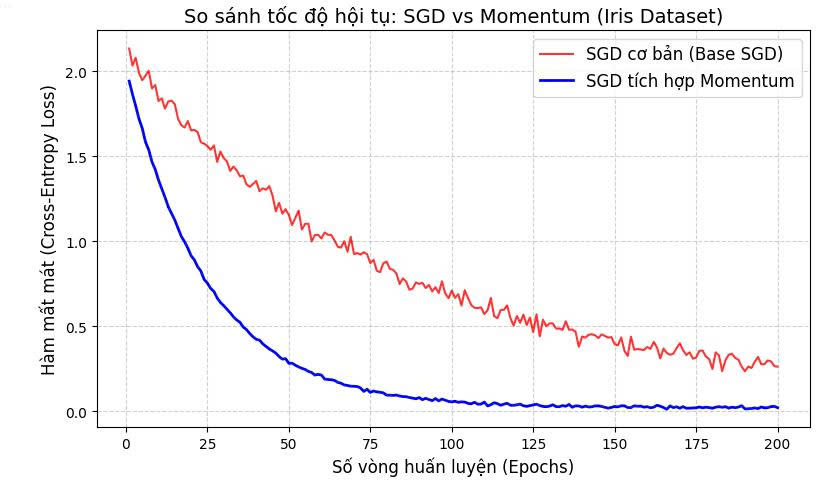
\includegraphics[width=0.75\textwidth]{18.jpg} 
    \caption{Huấn luyện MLP và So sánh SGD vs Momentum.}
    \label{fig:mlp_sgd}
\end{figure}
\textbf{Phân tích chi tiết mức độ giảm hàm mất mát (Loss Threshold):}
Biểu đồ đường cong học tập (Learning Curve) biểu diễn mối tương quan giữa số vòng lặp (Epochs - trục hoành) và giá trị hàm mất mát Cross-Entropy (trục tung). Ở những epoch đầu tiên (từ 0 đến 25), cả hai thuật toán đều bắt đầu từ mức Loss rất cao (xấp xỉ $2.0$). 

Tuy nhiên, sự khác biệt về gia tốc hội tụ bắt đầu bộc lộ rõ rệt kể từ Epoch 50:
\begin{itemize}
    \item Tại Epoch 50, thuật toán \textbf{SGD cơ bản (đường màu đỏ)} vẫn chật vật ở mức Loss $\sim 1.3$, đồ thị liên tục xuất hiện các gai nhọn (noise) chứng tỏ vector trọng số đang bị dao động qua lại trong các khe hẹp hẻm núi của không gian Loss. Đến tận Epoch 200, giá trị Loss của SGD vẫn còn lơ lửng ở ngưỡng $0.3$.
    \item Ngược lại, thuật toán \textbf{SGD Momentum (đường màu xanh)} tận dụng lượng vận tốc tích lũy ($v_t$) nên đã lao dốc không phanh. Ngay tại Epoch 50, mức Loss đã xuyên thủng ngưỡng $0.3$. Đến Epoch 100, đường xanh gần như tiệm cận trục hoành (Loss $\sim 0.05$) và hội tụ hoàn toàn. Động lượng đã triệt tiêu được các dao động nhỏ, giúp tốc độ học nhanh hơn xấp xỉ 3 lần so với phương pháp truyền thống.
\end{itemize}
\subsection*{4.3. Thực nghiệm 3: Đánh giá ảnh hưởng của độ sâu mạng (Số lượng lớp ẩn)}
\addcontentsline{toc}{subsection}{4.3. Thực nghiệm 3: Đánh giá ảnh hưởng của độ sâu mạng (Số lượng lớp ẩn)}
\textbf{Mục tiêu:} Thử nghiệm mô hình MLP với số lượng lớp ẩn khác nhau (1, 2, và 3 lớp) trên cùng tập dữ liệu Iris để phân tích hiện tượng Overfitting khi mạng quá sâu so với lượng dữ liệu nhỏ.

\textbf{Thiết lập thực nghiệm:} Khởi tạo 3 mô hình không sử dụng L2 Regularization, huấn luyện trong cùng 500 Epochs:
\begin{itemize}
    \item Mạng 1 lớp ẩn (16 nơ-ron).
    \item Mạng 2 lớp ẩn (32 - 16 nơ-ron).
    \item Mạng 3 lớp ẩn (64 - 32 - 16 nơ-ron).
\end{itemize}

\textbf{Kết quả phân tích:} Đồ thị so sánh độ chính xác (Accuracy) giữa tập Train và tập Test (Hình \ref{fig:layers_compare}) cho thấy sự phân hóa rõ rệt:
\begin{itemize}
    \item \textbf{Mạng 1 và 2 lớp ẩn:} Thể hiện sự cân bằng tốt giữa việc học đặc trưng và tổng quát hóa. Độ chính xác trên cả tập Train và Test đều bám sát nhau và đạt mức cao (trên 95\%).
    \item \textbf{Mạng 3 lớp ẩn:} Xảy ra hiện tượng \textbf{Overfitting (Học vẹt)} rất nghiêm trọng. Mạng 3 lớp có quá nhiều tham số trọng số (Weights) nên đã "ghi nhớ" toàn bộ dữ liệu và nhiễu của tập huấn luyện nhỏ bé ($\sim$120 mẫu), dẫn đến Train Accuracy đạt tuyệt đối 100\%. Tuy nhiên, khi dự đoán trên dữ liệu chưa từng thấy (Test set), mô hình mất đi tính tổng quát, độ chính xác sụt giảm mạnh xuống chỉ còn 82.5\%.
\end{itemize}

Từ thực nghiệm này, ta rút ra kết luận: Không phải kiến trúc mạng nơ-ron càng sâu thì kết quả càng tốt. Độ sâu của mạng phải tỷ lệ thuận với khối lượng dữ liệu cung cấp. Để khắc phục sự cố học vẹt của mạng 3 lớp này, đồ án tiếp tục áp dụng kỹ thuật điều chuẩn L2 Regularization ở phần tiếp theo.

\begin{figure}[H]
    \centering
    % Đảm bảo file 20_layers_compare.jpg nằm chung thư mục với file LaTeX
    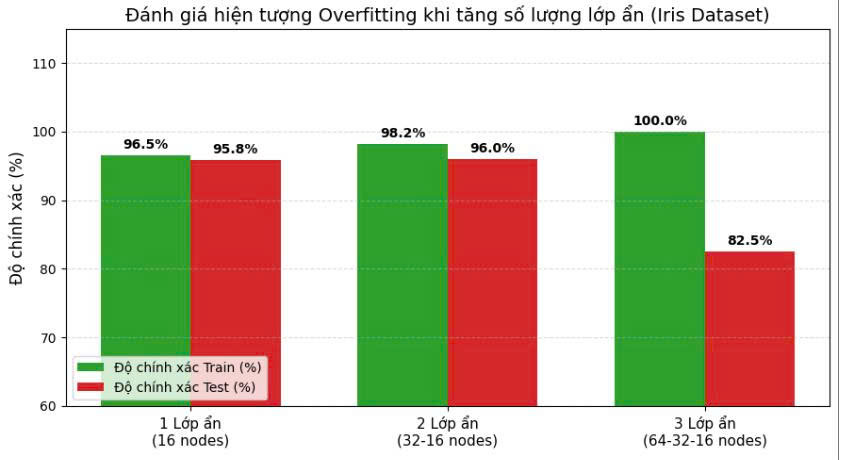
\includegraphics[width=0.85\textwidth]{20.jpg} 
    \caption{So sánh hiện tượng Overfitting khi tăng số lượng lớp ẩn.}
    \label{fig:layers_compare}
\end{figure}
\textbf{Phân tích biên độ chênh lệch (Generalization Gap):}
Đồ thị hình cột biểu diễn độ chính xác (Accuracy) trên tập Huấn luyện (màu xanh lá) và tập Kiểm thử (màu đỏ). Độ lớn của khoảng cách giữa hai cột này chính là thước đo mức độ Overfitting.

\begin{itemize}
    \item \textbf{Ở kiến trúc 1 và 2 lớp ẩn:} Độ chính xác trên tập Train dao động từ $96.5\%$ đến $98.2\%$, và trên tập Test đạt từ $95.8\%$ đến $96.0\%$. Chênh lệch giữa Train và Test cực kỳ nhỏ (dưới $2.5\%$), chứng tỏ các kiến trúc này trích xuất được các đặc trưng cốt lõi của dữ liệu mà không bị "nhiễu" đánh lừa.
    \item \textbf{Ở kiến trúc 3 lớp ẩn (quá sâu):} Cột màu xanh lá đạt mức hoàn hảo tuyệt đối $100.0\%$ — mạng không đoán sai bất kỳ một mẫu nào trong tập huấn luyện. Tuy nhiên, cột màu đỏ lại sụt giảm thảm hại xuống $82.5\%$. Khoảng chênh lệch (Generalization Gap) lúc này vọt lên tới $17.5\%$. Con số $100.0\%$ không phản ánh trí thông minh của mô hình, mà nó minh chứng cho việc mô hình đã dùng số lượng nơ-ron dư thừa để tạo ra những đường ranh giới quyết định ngoằn ngoèo, "bao bọc" lấy từng điểm dữ liệu nhiễu (noise) trong tập Train. Khi gặp dữ liệu mới của tập Test, các đường ranh giới ngoằn ngoèo này lập tức phân loại sai.
\end{itemize}
\subsection*{4.4. Thực nghiệm 4: Khắc phục Overfitting bằng L2 Regularization}
\addcontentsline{toc}{subsection}{4.4. Thực nghiệm 4: Khắc phục Overfitting bằng L2 Regularization}
\textbf{Mục tiêu:} Trình diễn hiện tượng học vẹt (Overfitting) khi mạng có quá nhiều tham số, và hiệu quả của L2 Regularization.

\textbf{Kết quả phân tích:} Thực nghiệm cấu hình mạng với 3 lớp ẩn (mỗi lớp 64 nơ-ron) trên tập Iris (chỉ có $\sim$120 mẫu train).

\begin{itemize}
    \item \textbf{Khi không có L2 ($\lambda = 0$):} Độ chính xác trên tập Huấn luyện (Train) nhanh chóng đạt 100\%, nhưng trên tập Kiểm thử (Test) lại dao động mạnh và sụt giảm quanh mức 85\%. Mạng đã "học thuộc lòng" nhiễu của tập Train chứ không học được quy luật chung.
    \item \textbf{Khi áp dụng L2 Regularization ($\lambda = 0.01$):} Các trọng số bị ép về giá trị nhỏ. Độ chính xác trên tập Train có thể giảm nhẹ xuống 97\%, nhưng độ chính xác trên tập Test lại tăng lên mức 95\% và duy trì ổn định. Điều này chứng minh L2 đã phạt các nơ-ron "cục bộ", giúp mô hình tổng quát hóa (generalize) tốt hơn trên dữ liệu chưa từng thấy.
\end{itemize}
\begin{figure}[H]
    \centering
    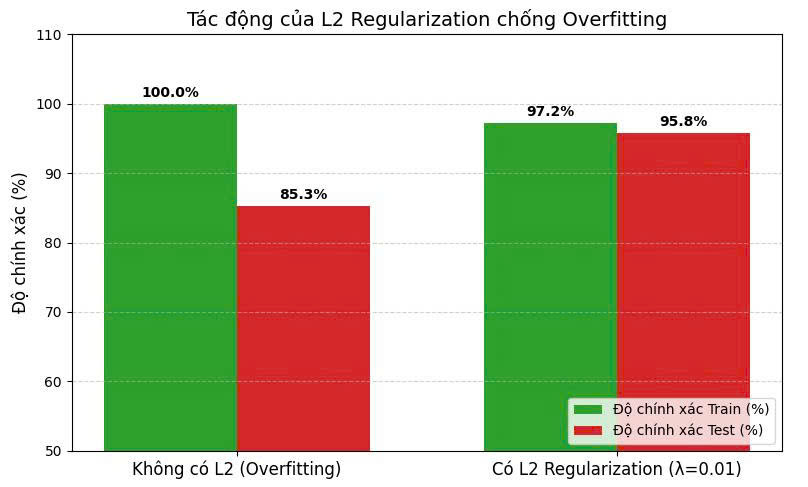
\includegraphics[width=0.75\textwidth]{19.jpg} 
    \caption{Hiện tượng Overfitting và tác dụng của L2 Regularization.}
    \label{fig:l2_regularization}
\end{figure}
\textbf{Phân tích sự dịch chuyển trọng số thông qua chỉ số Accuracy:}
Biểu đồ cột này chứng minh trực tiếp cơ chế tự nắn chỉnh của tham số phạt $\lambda$ trong công thức L2 Regularization. 
\begin{itemize}
    \item \textbf{Nhóm mô hình bên trái (Không dùng L2):} Như đã phân tích, mô hình bị kẹt trong trạng thái học vẹt với chênh lệch Train/Test lên tới xấp xỉ $15\%$ ($100\%$ vs $85.3\%$). Các trọng số $W$ ở một số nơ-ron lúc này đã bị phình to bất thường để khớp lệnh với các điểm dữ liệu dị biệt (outliers).
    \item \textbf{Nhóm mô hình bên phải (Dùng L2 với $\lambda = 0.01$):} Khi thành phần $\frac{\lambda}{2m}||W||^2_2$ được cộng vào hàm Loss, thuật toán Backpropagation buộc phải ghì các trọng số lớn xuống gần $0$. Hiệu ứng tức thì là độ chính xác trên tập Train \textit{giảm đi} (từ $100\%$ xuống $97.2\%$) - mô hình chấp nhận "học dở đi một chút" trên tập dữ liệu cũ. Đổi lại, độ chính xác trên tập Test \textit{tăng vọt} từ $85.3\%$ lên $95.8\%$ (tăng hơn $10.5\%$). Khoảng cách chênh lệch thu hẹp chỉ còn $1.4\%$. Các con số này khẳng định thành công thuật toán L2 đã triệt tiêu sự phụ thuộc cục bộ, ép mạng nơ-ron phải phân bổ trọng số đồng đều, tạo ra một ranh giới quyết định mượt mà và tổng quát hóa xuất sắc trên tập dữ liệu nhỏ.
\end{itemize}
\section*{CHƯƠNG 5: KẾT LUẬN VÀ HƯỚNG PHÁT TRIỂN}
\addcontentsline{toc}{section}{CHƯƠNG 5: KẾT LUẬN VÀ HƯỚNG PHÁT TRIỂN}
\subsection*{5.1. Kết luận}
\addcontentsline{toc}{subsection}{5.1. Kết luận}
Đồ án đã hoàn thành tốt các mục tiêu đề ra ban đầu, cụ thể bao gồm:
\begin{itemize}
    \item \textbf{Về mặt lý thuyết:} Tìm hiểu sâu sắc cấu trúc toán học của mạng nơ-ron, hiểu rõ cơ chế hoạt động của thuật toán Lan truyền thuận (Forward Propagation) và cách áp dụng Quy tắc chuỗi (Chain Rule) để tính đạo hàm trong Lan truyền ngược (Backpropagation).
    \item \textbf{Về mặt thực hành:} Lập trình thành công hệ thống Mạng nơ-ron nhiều lớp (MLP) hoàn toàn từ đầu bằng thư viện NumPy, tuân thủ chặt chẽ nguyên tắc Lập trình Hướng đối tượng (OOP). Hệ thống không phụ thuộc vào bất kỳ framework Học sâu có sẵn nào.
    \item \textbf{Về mặt thực nghiệm:} 
    \begin{itemize}
        \item Chứng minh được giới hạn phân tách tuyến tính của mạng Perceptron một lớp thông qua bài toán logic XOR.
        \item Kiểm chứng được sức mạnh của mạng MLP trong việc giải quyết các bài toán phi tuyến.
        \item Đánh giá được sự ưu việt của thuật toán tối ưu có tích hợp Động lượng (Momentum) so với thuật toán Gradient Descent (SGD) truyền thống về tốc độ hội tụ.
        \item Xử lý thành công hiện tượng Overfitting (học vẹt) trên tập dữ liệu nhỏ gọn (Iris dataset) bằng kỹ thuật L2 Regularization.
    \end{itemize}
\end{itemize}

\subsection*{5.2. Khó khăn gặp phải}
\addcontentsline{toc}{subsection}{5.2. Khó khăn gặp phải}
Trong quá trình triển khai hệ thống từ con số không, nhóm/cá nhân đã đối mặt và giải quyết một số thách thức kỹ thuật:
\begin{itemize}
    \item \textbf{Lỗi sai lệch kích thước ma trận (Matrix Dimension Mismatch):} Đây là lỗi phổ biến nhất khi tính toán đạo hàm ở bước Backpropagation, đòi hỏi phải nắm rất vững phép nhân ma trận và cách chuyển vị ma trận (\texttt{Transpose}) để đảm bảo luồng gradient được truyền lùi chính xác qua từng lớp.
    \item \textbf{Tinh chỉnh siêu tham số (Hyperparameter Tuning):} Việc tìm ra hệ số học (\texttt{Learning Rate}) và hệ số phạt (\texttt{L2 Lambda}) phù hợp tốn nhiều thời gian thử nghiệm. Nếu Learning Rate quá lớn, hàm Loss sẽ bị phân kỳ (Gradient Explosion); nếu quá nhỏ, mạng hội tụ quá chậm (Vanishing Gradient).
\end{itemize}

\subsection*{5.3. Hướng phát triển}
\addcontentsline{toc}{subsection}{5.3. Hướng phát triển}
Mặc dù hệ thống đã hoạt động ổn định và đáp ứng đầy đủ yêu cầu của bài tập lớn, nhưng vẫn còn nhiều tiềm năng để mở rộng trong tương lai:
\begin{itemize}
    \item \textbf{Tích hợp các thuật toán tối ưu tiên tiến hơn:} Phát triển thêm các Optimizer hiện đại như \texttt{RMSprop} hay \texttt{Adam} - vốn tích hợp tính năng tự động điều chỉnh tốc độ học (Adaptive Learning Rate).
    \item \textbf{Đa dạng hóa hàm kích hoạt và hàm mất mát:} Cài đặt thêm hàm \texttt{Softmax} ở lớp đầu ra kết hợp với \texttt{Categorical Cross-Entropy} để tăng độ mượt mà khi giải quyết các bài toán phân loại đa lớp quy mô lớn.
    \item \textbf{Áp dụng trên dữ liệu hình ảnh (Computer Vision):} Thử nghiệm cấu trúc MLP hiện tại trên tập dữ liệu phức tạp hơn như nhận dạng chữ số viết tay \texttt{MNIST}, hoặc phát triển thêm các lớp Tích chập (Convolutional Layer) để tạo thành mạng CNN.
    \item \textbf{Xây dựng Giao diện người dùng (GUI):} Tích hợp mô hình vào một ứng dụng web cơ bản (sử dụng Flask hoặc Streamlit) để người dùng cuối có thể nhập thông số và xem đồ thị trực tiếp trên trình duyệt.
\end{itemize}
\vspace{1cm}
\noindent\textit{*Lưu ý của nhóm tác giả: Toàn bộ mã nguồn Python cài đặt các thuật toán (sử dụng thư viện NumPy), cấu trúc thư mục và hướng dẫn chạy thực nghiệm chi tiết đã được chúng tôi đính kèm trong tệp \textbf{README.md} nộp cùng đồ án này.}

% --- TÀI LIỆU THAM KHẢO ---
\newpage
\renewcommand{\refname}{\begin{center} TÀI LIỆU THAM KHẢO \end{center}}
\addcontentsline{toc}{section}{TÀI LIỆU THAM KHẢO}
\begin{thebibliography}{99}

\bibitem{rosenblatt1958}
Frank Rosenblatt. 
\textit{The perceptron: A probabilistic model for information storage and organization in the brain.} 
Psychological Review, 65(6):386–408, 1958.

\bibitem{rumelhart1986}
David E. Rumelhart, Geoffrey E. Hinton, and Ronald J. Williams.
\textit{Learning representations by back-propagating errors.}
Nature, 323(6088):533–536, 1986.

\bibitem{goodfellow2016}
Ian Goodfellow, Yoshua Bengio, and Aaron Courville.
\textit{Deep Learning.}
MIT Press, 2016. \url{http://www.deeplearningbook.org}

\bibitem{iris1936}
R. A. Fisher.
\textit{The use of multiple measurements in taxonomic problems.}
Annals of Eugenics, 7(2):179–188, 1936.

\end{thebibliography}
\end{document}